\documentclass{article}
\usepackage{amsmath}
\usepackage{amsfonts}
\usepackage{tikz}
\usetikzlibrary{arrows}

\begin{document}

\begin{figure}[h]
    \centering
    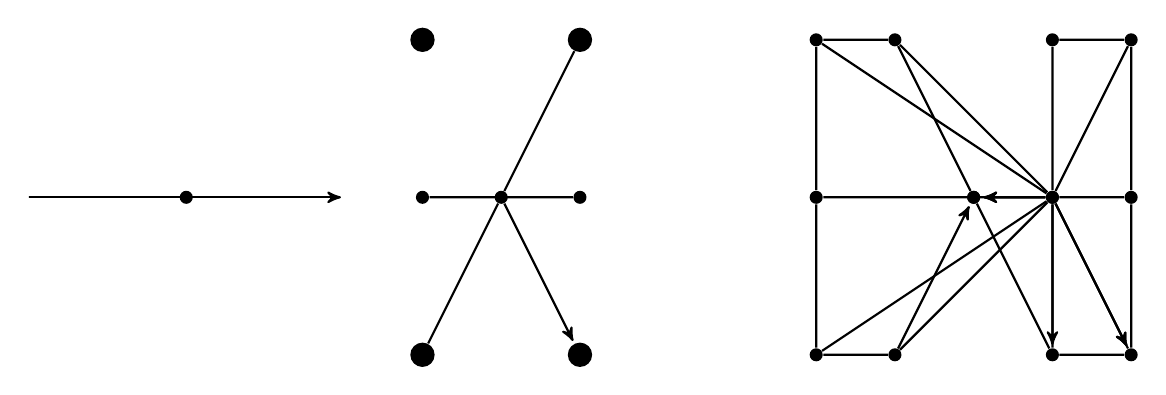
\begin{tikzpicture}[->,>=stealth',shorten >=1pt,auto,node distance=2cm,
        thick,main node/.style={circle,fill,scale=0.5}]
        
        % First graph
        \node[main node] (1) at (-4,0) {};
        \draw[] (1) -- +(-2,0) -- +(2,0);
        
        % Second graph
        \node[main node] (1) at (-1,0) {};
        \node[main node] (2) at (1,0) {};
        \node[main node] (3) at (-1,2) {1};
        \node[main node] (4) at (-1,-2) {2};
        \node[main node] (5) at (1,2) {5};
        \node[main node] (6) at (1,-2) {6};
        
        \node[main node] (3) at (0,0) {};
        \draw[] (3) -- (1) -- (2) -- (3) -- (4) -- (3) -- (5) -- (3) -- (6);
        
        % Third graph
        \node[main node] (7) at (7,2) {};
        \node[main node] (8) at (8,2) {};
        \node[main node] (9) at (8,0) {};
        \node[main node] (10) at (8,-2) {};
        \node[main node] (11) at (7,-2) {};
        \node[main node] (12) at (6,0) {};
        
        \node[main node] (13) at (5,2) {};
        \node[main node] (14) at (4,2) {};
        \node[main node] (15) at (4,0) {};
        \node[main node] (16) at (4,-2) {};
        \node[main node] (17) at (5,-2) {};
        \node[main node] (18) at (6,0) {};
        
        \node[main node] (19) at (7,0) {};
        \node[main node] (20) at (7,0) {};
        
        \draw[] (7) -- (8) -- (9) -- (10) -- (11) -- (12) -- (13) -- (14) -- (15) -- (16) -- (17) -- (18);
        \draw[] (7) -- (19) -- (14) -- (20) -- (11);
        \draw[] (8) -- (19) -- (15) -- (20) -- (10);
        \draw[] (9) -- (19) -- (16) -- (20) -- (10);
        \draw[] (10) -- (19) -- (17) -- (20) -- (12);
        \draw[] (11) -- (19) -- (13) -- (20) -- (12);
        
        \end{tikzpicture}
    \caption{Figure of the smallest replacement rule that produces a counter example to Conjecture \ref{conj:kleiner}. It is obtained from Example \ref{ex:laaksospace} by adding an edge to the vertex $v=3$ as in Lemma \ref{lem:removableedges}.}
    \label{fig:counterexample}
\end{figure}

\end{document}